% Options for packages loaded elsewhere
\PassOptionsToPackage{unicode}{hyperref}
\PassOptionsToPackage{hyphens}{url}
%
\documentclass[
  ignorenonframetext,
]{beamer}
\usepackage{pgfpages}
\setbeamertemplate{caption}[numbered]
\setbeamertemplate{caption label separator}{: }
\setbeamercolor{caption name}{fg=normal text.fg}
\beamertemplatenavigationsymbolsempty
% Prevent slide breaks in the middle of a paragraph
\widowpenalties 1 10000
\raggedbottom
\setbeamertemplate{part page}{
  \centering
  \begin{beamercolorbox}[sep=16pt,center]{part title}
    \usebeamerfont{part title}\insertpart\par
  \end{beamercolorbox}
}
\setbeamertemplate{section page}{
  \centering
  \begin{beamercolorbox}[sep=12pt,center]{part title}
    \usebeamerfont{section title}\insertsection\par
  \end{beamercolorbox}
}
\setbeamertemplate{subsection page}{
  \centering
  \begin{beamercolorbox}[sep=8pt,center]{part title}
    \usebeamerfont{subsection title}\insertsubsection\par
  \end{beamercolorbox}
}
\AtBeginPart{
  \frame{\partpage}
}
\AtBeginSection{
  \ifbibliography
  \else
    \frame{\sectionpage}
  \fi
}
\AtBeginSubsection{
  \frame{\subsectionpage}
}
\usepackage{amsmath,amssymb}
\usepackage{lmodern}
\usepackage{iftex}
\ifPDFTeX
  \usepackage[T1]{fontenc}
  \usepackage[utf8]{inputenc}
  \usepackage{textcomp} % provide euro and other symbols
\else % if luatex or xetex
  \usepackage{unicode-math}
  \defaultfontfeatures{Scale=MatchLowercase}
  \defaultfontfeatures[\rmfamily]{Ligatures=TeX,Scale=1}
\fi
\usefonttheme{structurebold}
% Use upquote if available, for straight quotes in verbatim environments
\IfFileExists{upquote.sty}{\usepackage{upquote}}{}
\IfFileExists{microtype.sty}{% use microtype if available
  \usepackage[]{microtype}
  \UseMicrotypeSet[protrusion]{basicmath} % disable protrusion for tt fonts
}{}
\makeatletter
\@ifundefined{KOMAClassName}{% if non-KOMA class
  \IfFileExists{parskip.sty}{%
    \usepackage{parskip}
  }{% else
    \setlength{\parindent}{0pt}
    \setlength{\parskip}{6pt plus 2pt minus 1pt}}
}{% if KOMA class
  \KOMAoptions{parskip=half}}
\makeatother
\usepackage{xcolor}
\newif\ifbibliography
\usepackage{longtable,booktabs,array}
\usepackage{calc} % for calculating minipage widths
\usepackage{caption}
% Make caption package work with longtable
\makeatletter
\def\fnum@table{\tablename~\thetable}
\makeatother
\usepackage{graphicx}
\makeatletter
\def\maxwidth{\ifdim\Gin@nat@width>\linewidth\linewidth\else\Gin@nat@width\fi}
\def\maxheight{\ifdim\Gin@nat@height>\textheight\textheight\else\Gin@nat@height\fi}
\makeatother
% Scale images if necessary, so that they will not overflow the page
% margins by default, and it is still possible to overwrite the defaults
% using explicit options in \includegraphics[width, height, ...]{}
\setkeys{Gin}{width=\maxwidth,height=\maxheight,keepaspectratio}
% Set default figure placement to htbp
\makeatletter
\def\fps@figure{htbp}
\makeatother
\setlength{\emergencystretch}{3em} % prevent overfull lines
\providecommand{\tightlist}{%
  \setlength{\itemsep}{0pt}\setlength{\parskip}{0pt}}
\setcounter{secnumdepth}{5}
\newlength{\cslhangindent}
\setlength{\cslhangindent}{1.5em}
\newlength{\csllabelwidth}
\setlength{\csllabelwidth}{3em}
\newlength{\cslentryspacingunit} % times entry-spacing
\setlength{\cslentryspacingunit}{\parskip}
\newenvironment{CSLReferences}[2] % #1 hanging-ident, #2 entry spacing
 {% don't indent paragraphs
  \setlength{\parindent}{0pt}
  % turn on hanging indent if param 1 is 1
  \ifodd #1
  \let\oldpar\par
  \def\par{\hangindent=\cslhangindent\oldpar}
  \fi
  % set entry spacing
  \setlength{\parskip}{#2\cslentryspacingunit}
 }%
 {}
\usepackage{calc}
\newcommand{\CSLBlock}[1]{#1\hfill\break}
\newcommand{\CSLLeftMargin}[1]{\parbox[t]{\csllabelwidth}{#1}}
\newcommand{\CSLRightInline}[1]{\parbox[t]{\linewidth - \csllabelwidth}{#1}\break}
\newcommand{\CSLIndent}[1]{\hspace{\cslhangindent}#1}
\usepackage{float}
\ifLuaTeX
  \usepackage{selnolig}  % disable illegal ligatures
\fi
\IfFileExists{bookmark.sty}{\usepackage{bookmark}}{\usepackage{hyperref}}
\IfFileExists{xurl.sty}{\usepackage{xurl}}{} % add URL line breaks if available
\urlstyle{same} % disable monospaced font for URLs
\hypersetup{
  pdftitle={Analyzing the influence of Selection on Genetic Programming's Generalization ability in Symbolic Regression},
  pdfauthor={Roman Hoehn, B.Sc. Wirtschaftspaedagogik},
  hidelinks,
  pdfcreator={LaTeX via pandoc}}

\title{Analyzing the influence of Selection on Genetic Programming's
Generalization ability in Symbolic Regression}
\subtitle{A comparison of epsilon-lexicase Selection and Tournament
Selection}
\author{Roman Hoehn, B.Sc. Wirtschaftspaedagogik}
\date{2022-06-29}

\begin{document}
\frame{\titlepage}

\begin{frame}[allowframebreaks]
  \tableofcontents[hideallsubsections]
\end{frame}
\hypertarget{introduction}{%
\section{Introduction}\label{introduction}}

\begin{frame}{Research Question}
\protect\hypertarget{research-question}{}
\begin{itemize}
\tightlist
\item
  Does the usage of \(\epsilon\)-lexicase parent selection influence the
  generalization behaviour of genetic programming in symbolic regression
  if compared to tournament selection?
\end{itemize}
\end{frame}

\begin{frame}{Genetic Programming}
\protect\hypertarget{genetic-programming}{}
\begin{itemize}
\tightlist
\item
  A metaheuristic that searches for computer programs that solve a given
  problem\footnote<.->{Koza (1992)}
\item
  Evolutionary Algorithm: Simulates the process of Darwinian evolution
\item
  Unique Features:

  \begin{itemize}
  \tightlist
  \item
    Evolve solutions of variable length and structure
  \item
    Solutions are typically represented by recursive tree structures
  \end{itemize}
\end{itemize}
\end{frame}

\begin{frame}{Parent Selection}
\protect\hypertarget{parent-selection}{}
\begin{block}{Torunament Selection}
\protect\hypertarget{torunament-selection}{}
\begin{itemize}
\tightlist
\item
  Most commonly used selection operator in Genetic Programming
  (GP)\footnote<.->{Fang and Li (2010), p.181}
\item
  Intuition: High chance for ``generalist'' solutions to be selected
  since it is based on aggregated fitness scores
\end{itemize}
\end{block}

\begin{block}{\(\epsilon\)-Lexicase Selection}
\protect\hypertarget{epsilon-lexicase-selection}{}
\begin{itemize}
\tightlist
\item
  Objective: Create Selection method for uncompromising,
  continous-valued symbolic regression problems \footnote<.->{Helmuth,
    Spector and Matheson (2015), p.12}
\item
  Performance increases have been demonstrated in many benchmarking
  problems \footnote<.->{La Cava, Spector and Danai (2016), p.744-745}
\item
  Intuition: Higher chance for ``specialist'' solutions to be selected
  since it is decided on a per case basis
\end{itemize}
\end{block}
\end{frame}

\begin{frame}{Related Concepts}
\protect\hypertarget{related-concepts}{}
\begin{block}{Symbolic Regression}
\protect\hypertarget{symbolic-regression}{}
\begin{itemize}
\tightlist
\item
  Task: Find a mathematical model that fits a given set of datapoints
\item
  One of the first applications of GP described by Koza (1992)
\item
  High relevance: GP can outperform state-of-the-art machine learning
  algorithms like gradient boosting \footnote<.->{Orzechowski, Cava and
    Moore (2018)}
\end{itemize}
\end{block}

\begin{block}{Generalization}
\protect\hypertarget{generalization}{}
\begin{itemize}
\tightlist
\item
  Main objective in most supervised machine learning problems: Achieve
  good performance for unseen data
\item
  Challenge: Avoid overfitting to training data
\item
  Little attention has been paid to generalization in GP \footnote<.->{O'Neill
    \emph{et al.} (2010), Kushchu (2002)}
\end{itemize}
\end{block}
\end{frame}

\hypertarget{experimental-study}{%
\section{Experimental Study}\label{experimental-study}}

\begin{frame}{Benchmark problem}
\protect\hypertarget{benchmark-problem}{}
UC Irvine Machine Learning Repository: Prediction of energy efficiency
in buildings \footnote<.->{Dua and Graff (2017)}

\begin{longtable}[]{@{}ll@{}}
\caption{Overview - Energy Heating data set}\tabularnewline
\toprule()
Variable & Description \\
\midrule()
\endfirsthead
\toprule()
Variable & Description \\
\midrule()
\endhead
X1 & Relative Compactness \\
X2 & Surface Area \\
X3 & Wall Area \\
X4 & Roof Area \\
X5 & Overall Height \\
X6 & Orientation \\
X7 & Glazing Area \\
X8 & Glazing Area Distribution \\
y1 & Heating Load \\
y2 & Cooling Load \\
\bottomrule()
\end{longtable}
\end{frame}

\begin{frame}{Experiment}
\protect\hypertarget{experiment}{}
\begin{block}{Single run}
\protect\hypertarget{single-run}{}
\begin{itemize}
\tightlist
\item
  Total dataset (\(N=768\)) is randomly split into a training and
  testing dataset (50:50)
\item
  Fitness metric: Mean squared Error (MSE)
\item
  Train two models using GP with the training dataset only, one using
  tournament selection and the other \(\epsilon\)-lexicase selection
\item
  For each generation: Select elite model and compute its fitness for
  the testing dataset
\end{itemize}
\end{block}

\begin{block}{Full experiment}
\protect\hypertarget{full-experiment}{}
\begin{itemize}
\tightlist
\item
  Stochastic algorithm: Repeat the basic experiment for 50 total runs
\item
  Collect and aggregate results for training error, testing error and
  program length
\end{itemize}
\end{block}
\end{frame}

\begin{frame}{Hypothesis Testing}
\protect\hypertarget{hypothesis-testing}{}
\textbf{Does the usage of \(\epsilon\)-lexicase parent selection
influence the generalization behavior of genetic programming in symbolic
regression if compared to tournament selection?}

\begin{enumerate}
\tightlist
\item
  Test for differences in average fitness between both algorithms
\item
  Test for differences in average fitness between training and testing
  data
\end{enumerate}
\end{frame}

\hypertarget{results}{%
\section{Results}\label{results}}

\begin{frame}{Finding 1}
\protect\hypertarget{finding-1}{}
\begin{itemize}
\tightlist
\item
  The differences in average fitness of the final solutions between
  tournament selection and \(\epsilon\)-lexicase selection are highly
  statistical significant (\(\alpha=0.01\))
\item
  Tournament selection-based GP achieves a higher fitness for both
  training and testing data
\item
  Unexpected results based on the reviewed literature (La Cava, Spector
  and Danai, 2016), (La Cava \emph{et al.}, 2017)
\end{itemize}
\end{frame}

\begin{frame}{Distribution of Fitness}
\protect\hypertarget{distribution-of-fitness}{}
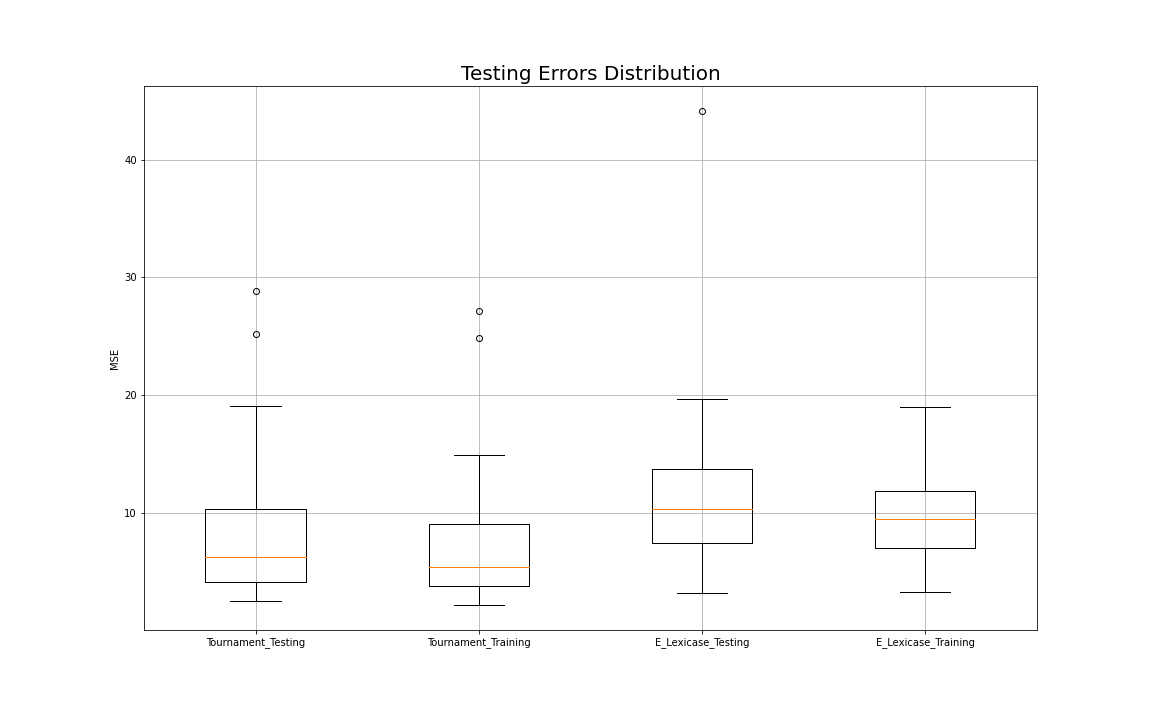
\includegraphics{../plots/mean_error_boxplot_all.png}
\end{frame}

\begin{frame}{Example}
\protect\hypertarget{example}{}
Model evolved by tournament selection after 100 generations:

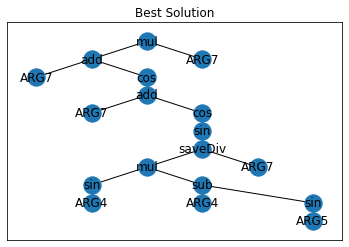
\includegraphics{../plots/example_model.png}
\end{frame}

\begin{frame}{Finding 2}
\protect\hypertarget{finding-2}{}
\begin{itemize}
\tightlist
\item
  The gap between training and testing error is not statistically
  significant for both selection algorithms
\item
  Both algorithms achieve a slightly better performance for the training
  data
\item
  Good generalization: No evidence of overfitting
\end{itemize}
\end{frame}

\begin{frame}{Evolution of Fitness}
\protect\hypertarget{evolution-of-fitness}{}
\includegraphics{../plots/mean_error_combined.png}
\end{frame}

\begin{frame}{Statistical Test}
\protect\hypertarget{statistical-test}{}
\begin{table}

\caption{\label{tab:pvals_fitness}Mean Error - P-Values (MWU)}
\centering
\fontsize{4}{6}\selectfont
\begin{tabular}[t]{l|r|r|r|r}
\hline
X & tournament\_training\_errors & tournament\_testing\_errors & elexicase\_training\_errors & elexicase\_testing\_errors\\
\hline
tournament\_training\_errors & 1.000 & 0.309 & 0.000 & 0.000\\
\hline
tournament\_testing\_errors & 0.309 & 1.000 & 0.002 & 0.000\\
\hline
elexicase\_training\_errors & 0.000 & 0.002 & 1.000 & 0.257\\
\hline
elexicase\_testing\_errors & 0.000 & 0.000 & 0.257 & 1.000\\
\hline
\end{tabular}
\end{table}
\end{frame}

\begin{frame}{Program Growth}
\protect\hypertarget{program-growth}{}
\begin{itemize}
\tightlist
\item
  So far: No proof of differences in generalization
\item
  New approach: Program growth as a possible indicator for overfitting?
\item
  Theory: Minimum description length principle (MDLP) \footnote<.->{Wang,
    Wagner and Rondinelli (2019), p.~268}
\item
  Downside: Growth/Bloat is no clear indicator of overfitting
  \footnote<.->{Silva and Vanneschi (2009), p.~8}
\end{itemize}
\end{frame}

\begin{frame}{Evolution of Size}
\protect\hypertarget{evolution-of-size}{}
\begin{figure}
\centering
\includegraphics{../plots/size_subplotted.png}
\end{figure}
\end{frame}

\begin{frame}{Finding 3}
\protect\hypertarget{finding-3}{}
\begin{itemize}
\tightlist
\item
  GP typical growth behaviour for both operators
\item
  Solutions grow at a similiar rate in each generation
\item
  No statistically significant differences in overall program size based
  on selection
\end{itemize}
\end{frame}

\hypertarget{conclusions}{%
\section{Conclusions}\label{conclusions}}

\begin{frame}{Conclusions}
\begin{itemize}
\tightlist
\item
  Experiment did not yield evidence for differences in generalization
  behavior between tournament and \(\epsilon\)-lexicase selection
\item
  The performance of tournament selection is significantly higher than
  that of \(\epsilon\)-lexicase selection for the selected symbolic
  regression problem
\item
  No evidence for differences in growth behavior between both algorithms
\end{itemize}
\end{frame}

\hypertarget{limitations-and-open-questions}{%
\section{Limitations and open
Questions}\label{limitations-and-open-questions}}

\begin{frame}{Limitations and open Questions}
\begin{enumerate}
\tightlist
\item
  Configuration of evolutionary parameters
\item
  Results are based on a single symbolic regression
\item
  Limited by computational resources
\end{enumerate}
\end{frame}

\hypertarget{appendix}{%
\section{Appendix}\label{appendix}}

\begin{frame}{Evolutionary Parameters}
\protect\hypertarget{evolutionary-parameters}{}
\begin{table}

\caption{\label{tab:ea_config}Evolutionary Parameters}
\centering
\begin{tabular}[t]{l|l}
\hline
Parameter & Value\\
\hline
Population Size & 500\\
\hline
Number of Generations & 100\\
\hline
Mutation Rate & 20\%\\
\hline
Crossover Rate & 80\%\\
\hline
Tournament Size & 3\\
\hline
Epsilon selection & automatic\\
\hline
Elite Size & 0\\
\hline
\end{tabular}
\end{table}
\end{frame}

\begin{frame}[allowframebreaks]{Primitive Set}
\protect\hypertarget{primitive-set}{}
\begin{table}

\caption{\label{tab:primitive_table}Function Set}
\centering
\begin{tabular}[t]{l|r}
\hline
Function & Arity\\
\hline
Addition & 2\\
\hline
Subtraction & 2\\
\hline
Multiplication & 2\\
\hline
Negation & 1\\
\hline
Sine & 1\\
\hline
Cosine & 1\\
\hline
Protected Division & 2\\
\hline
Protected Natural Logarithm & 1\\
\hline
Protected Square Root & 1\\
\hline
\end{tabular}
\end{table}
\framebreak

\begin{table}

\caption{\label{tab:function_table}Terminal Set}
\centering
\begin{tabular}[t]{l|l}
\hline
Terminal & Description\\
\hline
X1 & Relative Compactness\\
\hline
X2 & Surface Area\\
\hline
X3 & Wall Area\\
\hline
X4 & Roof Area\\
\hline
X5 & Overall Height\\
\hline
X6 & Orientation\\
\hline
X7 & Glazing Area\\
\hline
X8 & Glazing Area Distribution\\
\hline
random\_int & Ephemeral Constant (integer)\\
\hline
random\_float & Ephemeral Constant(float)\\
\hline
\end{tabular}
\end{table}
\end{frame}

\hypertarget{references}{%
\section*{References}\label{references}}
\addcontentsline{toc}{section}{References}

\begin{frame}[allowframebreaks]{References}
\hypertarget{refs}{}
\begin{CSLReferences}{0}{0}
\leavevmode\vadjust pre{\hypertarget{ref-Dua:2019}{}}%
Dua, D. and Graff, C. (2017) {``{UCI} machine learning repository.''}
University of California, Irvine, School of Information; Computer
Sciences. Available at: \url{http://archive.ics.uci.edu/ml}.

\leavevmode\vadjust pre{\hypertarget{ref-10.1007ux2f978-3-642-16493-4_19}{}}%
Fang, Y. and Li, J. (2010) {``A review of tournament selection in
genetic programming,''} in Cai, Z. et al. (eds.) \emph{Advances in
computation and intelligence}. Berlin, Heidelberg: Springer Berlin
Heidelberg, pp. 181--192.

\leavevmode\vadjust pre{\hypertarget{ref-6920034}{}}%
Helmuth, T., Spector, L. and Matheson, J. (2015) {``Solving
uncompromising problems with lexicase selection,''} \emph{IEEE
Transactions on Evolutionary Computation}, 19(5), pp. 630--643.
doi:\href{https://doi.org/10.1109/TEVC.2014.2362729}{10.1109/TEVC.2014.2362729}.

\leavevmode\vadjust pre{\hypertarget{ref-koza_main}{}}%
Koza, J.R. (1992) \emph{Genetic programming: On the programming of
computers by means of natural selection}. Cambridge, MA, USA: MIT Press.
Available at: \url{http://mitpress.mit.edu/books/genetic-programming}.

\leavevmode\vadjust pre{\hypertarget{ref-generalisation_in_gp}{}}%
Kushchu, I. (2002) {``An evaluation of EvolutionaryGeneralisation in
genetic programming,''} \emph{Artificial Intelligence Review - AIR}, 18,
pp. 3--14.
doi:\href{https://doi.org/10.1023/A:1016379201230}{10.1023/A:1016379201230}.

\leavevmode\vadjust pre{\hypertarget{ref-https:ux2fux2fdoi.orgux2f10.48550ux2farxiv.1709.05394}{}}%
La Cava, W. \emph{et al.} (2017) {``A probabilistic and multi-objective
analysis of lexicase selection and epsilon-lexicase selection.''} arXiv.
doi:\href{https://doi.org/10.48550/ARXIV.1709.05394}{10.48550/ARXIV.1709.05394}.

\leavevmode\vadjust pre{\hypertarget{ref-epsilon_lexicase_main}{}}%
La Cava, W., Spector, L. and Danai, K. (2016) {``Epsilon-lexicase
selection for regression,''} in \emph{Proceedings of the genetic and
evolutionary computation conference 2016}. New York, NY, USA:
Association for Computing Machinery (GECCO '16), pp. 741--748.
doi:\href{https://doi.org/10.1145/2908812.2908898}{10.1145/2908812.2908898}.

\leavevmode\vadjust pre{\hypertarget{ref-open_issues_gp}{}}%
O'Neill, M. \emph{et al.} (2010) {``Open issues in genetic
programming,''} \emph{Genetic Programming and Evolvable Machines}, 11,
pp. 339--363.
doi:\href{https://doi.org/10.1007/s10710-010-9113-2}{10.1007/s10710-010-9113-2}.

\leavevmode\vadjust pre{\hypertarget{ref-Orzechowski_2018}{}}%
Orzechowski, P., Cava, W.L. and Moore, J.H. (2018) {``Where are we
now?''} in \emph{Proceedings of the genetic and evolutionary computation
conference}. {ACM}.
doi:\href{https://doi.org/10.1145/3205455.3205539}{10.1145/3205455.3205539}.

\leavevmode\vadjust pre{\hypertarget{ref-bloat_overfitting_gp}{}}%
Silva, S. and Vanneschi, L. (2009) {``Operator equalisation, bloat and
overfitting: A study on human oral bioavailability prediction,''} in
\emph{Proceedings of the 11th Annual Genetic and Evolutionary
Computation Conference, GECCO-2009}, pp. 1115--1122.
doi:\href{https://doi.org/10.1145/1569901.1570051}{10.1145/1569901.1570051}.

\leavevmode\vadjust pre{\hypertarget{ref-wang_wagner_rondinelli_2019}{}}%
Wang, Y., Wagner, N. and Rondinelli, J.M. (2019) {``Symbolic regression
in materials science,''} \emph{MRS Communications}, 9(3), pp. 793--805.
doi:\href{https://doi.org/10.1557/mrc.2019.85}{10.1557/mrc.2019.85}.

\end{CSLReferences}
\end{frame}

\end{document}
